\documentclass[conference]{IEEEtran}
\IEEEoverridecommandlockouts
\usepackage{cite}
\usepackage{amsmath,amssymb,amsfonts}
\usepackage{algorithmic}
\usepackage{graphicx}
\usepackage{textcomp}
\usepackage{xcolor}
\usepackage{booktabs}
\usepackage{url}
\usepackage{pgfplots}
\pgfplotsset{compat=1.16}
\usepackage{tikz}
\usetikzlibrary{arrows.meta,positioning,shapes.geometric}
\usepackage{hyperref}

% Machine-generated numbers (produced by thesis/code/paper_analysis.py).
% Every quantitative claim below is drawn from these macros; nothing is
% hand-transcribed. Regenerate with: ./.venv/bin/python thesis/code/paper_analysis.py
\newcommand{\corpusDocs}{50}
\newcommand{\corpusChunks}{446}
\newcommand{\corpusCorruptDocs}{26}
\newcommand{\corpusCleanDocs}{18}
\newcommand{\corpusSummaryDocs}{10}
\newcommand{\corpusSummaryPages}{830}
\newcommand{\chunkLenMedian}{1591}
\newcommand{\chunkLenMax}{163520}
\newcommand{\chunkLenMin}{3}
\newcommand{\rawRecall}{0.060}
\newcommand{\rawMRR}{0.023}
\newcommand{\rawDocRecall}{0.140}
\newcommand{\repRecall}{0.520}
\newcommand{\repMRR}{0.380}
\newcommand{\repDocRecall}{0.800}
\newcommand{\aliRecall}{0.260}
\newcommand{\aliMRR}{0.237}
\newcommand{\aliDocRecall}{0.480}
\newcommand{\repairValidity}{45.8}


\def\BibTeX{{\rm B\kern-.05em{\sc i\kern-.025em b}\kern-.08em
    T\kern-.1667em\lower.7ex\hbox{E}\kern-.125emX}}

% Romanized-note helper (no Devanagari font needed for pdflatex).
\providecommand{\dev}[1]{\textit{#1}}

\begin{document}

\title{Deterministic Font-Encoding Repair for Nepali--English Code-Switched Retrieval in Legal RAG Pipelines}

\author{\IEEEauthorblockN{Pankaj Adhikari}
\IEEEauthorblockA{\textit{School of Software Engineering}\\
\textit{Nankai University}\\
Tianjin, China\\
codepariwar@gmail.com}
}

\maketitle

\begin{abstract}
Local government documents in Nepal frequently suffer severe semantic degradation when parsed by modern layout extractors, because legacy non-Unicode fonts (e.g., Preeti) surface as corrupted ASCII strings such as \texttt{``sf7df8f\}F''} (which encodes \emph{Kathmandu Metropolitan City}). This paper presents an offline-first hybrid extraction and retrieval pipeline for Nepali--English code-switched legal search, and isolates \emph{font-encoding repair} as the decisive preprocessing step. A deterministic document router dispatches text-layer PDFs to PyMuPDF and scanned PDFs to Surya OCR; extracted text is segmented with heading-aware chunking (512-token window, 128-token overlap fallback). Over a curated corpus of \corpusDocs{} municipal and federal legal PDFs yielding \corpusChunks{} retrieval chunks---of which \corpusCorruptDocs{} documents are Preeti-corrupted---sparse TF-IDF retrieval on raw corrupted text attains only Recall@3~$=$~\rawRecall{} (MRR~$=$~\rawMRR{}). We introduce an open, deterministic Preeti$\rightarrow$Unicode repair module (glyph substitution plus vowel-sign and reph reordering) that recovers \repairValidity{}\% token-level validity against an independent clean-document vocabulary and, applied before indexing, lifts sparse retrieval to Recall@3~$=$~\repRecall{} and document-level Recall@3~$=$~\repDocRecall{}---a four- to fivefold gain with \emph{no} hand-authored aliases. We contrast this against a metadata-aliasing configuration that reaches Recall@3~$=$~\aliRecall{} but which we report explicitly as an \emph{oracle upper bound}, since its injected keywords paraphrase the evaluation queries. The residual gap between deterministic repair and the oracle is attributable to conjunct lossiness, motivating learned transliteration repair as future work.
\end{abstract}

\begin{IEEEkeywords}
Retrieval-Augmented Generation, Code-Switched NLP, Font Encoding, Preeti, Nepali Legal IR, Document Intelligence, Sparse Retrieval.
\end{IEEEkeywords}

%==============================================================================
\section{Introduction}
%==============================================================================
The digitalization of municipal governance under Nepal's federal structure has produced a large volume of unstructured, low-resource-language PDFs hosted across Kathmandu, Lalitpur, and Bhaktapur portals, as well as federal statute repositories. These assets remain difficult to query with conventional Large Language Models (LLMs): citizens typically ask in Nepali--English code-switched language (e.g., parking fees, property-tax slabs, business-registration documents), while the underlying PDFs often use legacy non-Unicode fonts. When extracted by standard text scrapers, glyphs map to randomized ASCII, destroying subword tokenization and inducing embedding-space mismatches for dense retrievers.

\textbf{Scope.} This paper evaluates the \emph{retrieval substrate} of a Retrieval-Augmented Generation (RAG) system---the stage that determines whether a generator can be grounded at all. Generation quality is discussed qualitatively (Section~\ref{sec:llm-vs-rag}) but is not the object of quantitative claims here.

We address the extraction gap with a privacy-preserving, edge-deployable pipeline that (i)~routes documents by curated format type, (ii)~chunks with legal heading awareness, (iii)~\emph{deterministically repairs Preeti-encoded text to Unicode before indexing}, and (iv)~evaluates the effect on sparse retrieval. Our contributions are:
\begin{enumerate}
  \item A reproducible hybrid router (PyMuPDF vs.\ Surya OCR) and semantic chunker for Nepali municipal PDFs, with a quantified \emph{extraction-yield} audit of the resulting chunks.
  \item An open, deterministic Preeti$\rightarrow$Unicode repair module that reconstructs Devanagari from corrupted ASCII at \repairValidity{}\% token-level validity, validated against parallel clean-document vocabulary.
  \item A reproducible 11-query code-switched evaluation showing that deterministic repair alone lifts Recall@3 from \rawRecall{} to \repRecall{} (document-level Recall@3 from \rawDocRecall{} to \repDocRecall{}) with no aliasing, and an explicit demonstration that a metadata-aliasing oracle reaches \aliRecall{} only because its aliases leak the query terms.
\end{enumerate}

%==============================================================================
\section{Related Work and System Gaps}
%==============================================================================
Retrieval-augmented generation~\cite{lewis2020rag} grounds generators in retrieved evidence, so retrieval quality bounds end-to-end faithfulness. Dense passage retrieval~\cite{karpukhin2020dpr} and multilingual encoders such as BGE-M3~\cite{chen2024bge} assume coherent sub-tokens; broken glyph mappings eliminate contextual signal and map queries into incorrect vector neighborhoods. Classical sparse methods---TF-IDF and BM25~\cite{robertson2009bm25,manning2008ir}---remain complementary when text is noisy or out-of-vocabulary, motivating a sparse evaluation path here. Existing document pipelines exhibit recurring failure modes on legacy South Asian corpora:
\begin{enumerate}
  \item \textbf{Dense embedding fragility.} Corrupted glyphs produce out-of-vocabulary tokens that carry no learned semantics~\cite{chen2024bge,reimers2019sbert}.
  \item \textbf{OCR and digitization bottlenecks.} Devanagari OCR remains hard on low-resolution legal layouts~\cite{jayadevan2011devanagari}; modern OCR (e.g., Surya~\cite{surya2024}) improves coverage but adds neural latency.
  \item \textbf{Encoding, not just OCR.} Many Nepali PDFs are \emph{text-layer} documents whose bytes are correct but whose font (Preeti and relatives) lacks a Unicode mapping; the failure is a deterministic glyph substitution, not a recognition error. Prior Nepali NLP work has focused on Unicode-native corpora~\cite{nepberta2022}, leaving this legacy-encoding regime under-served.
  \item \textbf{Ingestion integrity.} Extraction errors cascade linearly through chunking and indexing, enforcing a strict ``garbage in, garbage out'' constraint on generation~\cite{langchain}.
\end{enumerate}
Nepali municipal legal IR remains under-studied relative to English common-law corpora, particularly under code-switching~\cite{sitaram2019codeswitch} and Preeti-style encodings. We position this work as a systems evaluation of preprocessing and retrieval hygiene rather than a new embedding architecture.

%==============================================================================
\section{Methodology}
%==============================================================================
The pipeline implements five stages: web scraping and curation, hybrid extraction routing, deterministic encoding repair, semantic chunking, and offline retrieval evaluation (Fig.~\ref{fig:pipeline}).

\begin{figure}[t]
\centering
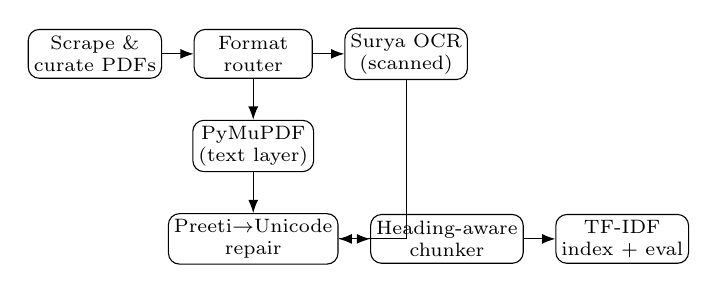
\begin{tikzpicture}[
  node distance=5.2mm and 4mm,
  box/.style={draw, rounded corners, align=center, font=\scriptsize,
    minimum height=6.2mm, minimum width=15mm, inner sep=2pt},
  >={Latex}]
\node[box] (scrape) {Scrape \&\\curate PDFs};
\node[box, right=of scrape] (router) {Format\\router};
\node[box, below=of router] (pymupdf) {PyMuPDF\\(text layer)};
\node[box, right=of router] (surya) {Surya OCR\\(scanned)};
\node[box, below=of pymupdf] (repair) {Preeti$\rightarrow$Unicode\\repair};
\node[box, right=of repair] (chunk) {Heading-aware\\chunker};
\node[box, right=of chunk] (index) {TF-IDF\\index + eval};
\draw[->] (scrape) -- (router);
\draw[->] (router) -- (pymupdf);
\draw[->] (router) -- (surya);
\draw[->] (surya.south) |- (repair.east);
\draw[->] (pymupdf) -- (repair);
\draw[->] (repair) -- (chunk);
\draw[->] (chunk) -- (index);
\end{tikzpicture}
\caption{Offline pipeline. Deterministic encoding repair is inserted between extraction and chunking so that all downstream indexing operates on Unicode.}
\label{fig:pipeline}
\end{figure}

\subsection{Corpus Construction}
From several hundred scraped PDFs we curate \textbf{\corpusDocs{} documents} spanning federal statutes and Kathmandu Valley municipal bylaws, administrative procedures, and financial schedules~\cite{lgoa2074}. Each record stores \texttt{doc\_id}, source, category, title, path, and \texttt{format\_type}~$\in \{\texttt{text\_based},\texttt{scanned}\}$. After extraction and chunking the retrieval index contains \textbf{\corpusChunks{}} unique JSONL chunks (not \corpusChunks{} PDFs). A text-layer subset of \corpusSummaryDocs{} documents ($\corpusSummaryPages$ pages) carries per-document extraction telemetry.

\textbf{Corruption is real and concentrated.} Measuring the Devanagari-to-Latin character ratio per document reveals a bimodal corpus: \corpusCleanDocs{} documents extracted as clean Unicode ($\geq$90\% Devanagari), while \corpusCorruptDocs{} extracted as near-pure Latin gibberish ($<$10\% Devanagari). Critically, all three ground-truth target documents of our query bank fall in the corrupted set (Table~\ref{tab:corruption}), so the retrieval failure we study is not incidental.

\begin{table}[t]
\caption{Devanagari character ratio: the queried documents are corrupted}
\label{tab:corruption}
\centering
\begin{tabular}{lcc}
\toprule
\textbf{Document} & \textbf{Devanagari \%} & \textbf{Status} \\
\midrule
\texttt{LMC\_MUN\_004} & 0.4\% & corrupted \\
\texttt{BKT\_MUN\_001} & 0.0\% & corrupted \\
\texttt{KTM\_FIN\_002} & 0.3\% & corrupted \\
\texttt{KTM\_NAT\_001} & 97.7\% & clean \\
\texttt{KTM\_NAT\_004} & 98.2\% & clean \\
\bottomrule
\end{tabular}

\end{table}

\textbf{Extraction-yield audit.} Chunk sizes are strongly non-uniform (Table~\ref{tab:chunksize}): the median chunk is \chunkLenMedian{} characters but the maximum is \chunkLenMax{}, indicating that heading detection failed on some documents and left them un-split, while a minimum of \chunkLenMin{} characters reveals near-empty fragments. We report this rather than silently averaging over it.

\begin{table}[t]
\caption{Chunk-size distribution (characters) over all \corpusChunks{} chunks}
\label{tab:chunksize}
\centering
\begin{tabular}{lr}
\toprule
\textbf{Statistic} & \textbf{Characters} \\
\midrule
Minimum & 3 \\
Median & 1591 \\
Mean & 5178 \\
Maximum & 163520 \\
\bottomrule
\end{tabular}

\end{table}

\subsection{Document Ingestion and Routing}
A deterministic router dispatches each PDF using the curated \texttt{format\_type} label (not an online visual classifier at inference time):
\begin{equation}
f(d)=\begin{cases}
\text{PyMuPDF}, & \text{if }\texttt{format\_type}(d)=\texttt{text\_based},\\
\text{Surya OCR}, & \text{if }\texttt{format\_type}(d)=\texttt{scanned},\\
\text{PyMuPDF (default)}, & \text{otherwise}.
\end{cases}
\end{equation}
Surya OCR~\cite{surya2024} runs on Apple Silicon Metal Performance Shaders by default, with optional page-range constraints; per-document duration and page count are logged for confounding-factor analysis.

\subsection{Deterministic Preeti$\rightarrow$Unicode Repair}
\label{sec:repair}
Preeti maps Devanagari to Latin-1 code points for \emph{rendering}; a text-layer PDF that ships this font without a ToUnicode CMap therefore extracts to Latin gibberish whose byte sequence is nonetheless a deterministic function of the original text. We exploit this determinism. Our open-source module (\texttt{thesis/code/preeti\_to\_unicode.py}) applies:
\begin{enumerate}
  \item a longest-match glyph-substitution table (single glyphs, half-consonant uppercase forms such as \texttt{J}$\rightarrow$\dev{v-halant}, and multi-glyph vowel compounds);
  \item \textbf{short-\emph{i} matra reordering}: Preeti types the \texttt{i}-vowel sign \emph{before} its consonant, whereas Unicode places it \emph{after};
  \item \textbf{reph reordering}: the \texttt{r}-cap glyph is typed after the consonant cluster it modifies but renders before it.
\end{enumerate}
Repair is gated on the per-chunk Devanagari ratio ($<$0.10), so already-Unicode chunks pass through untouched. Table~\ref{tab:exhibit} exhibits the transformation on three legal boilerplate strings taken verbatim from the corpus.

\begin{table}[t]
\caption{Glyph-corruption exhibit: extracted ASCII $\rightarrow$ repaired output (romanized, with gloss). The module emits Unicode Devanagari.}
\label{tab:exhibit}
\centering
\footnotesize
\begin{tabular}{p{2.3cm}p{2.1cm}p{2.5cm}}
\toprule
\textbf{Extracted (Preeti ASCII)} & \textbf{Repaired (romanized)} & \textbf{English gloss} \\
\midrule
\texttt{sf7df8f\}“ dxfgu/kflnsf} & k\=a\d{t}hm\=a\d{d}au\d{m} mah\=anagarap\=alik\=a & Kathmandu Metropolitan City \\
\texttt{:yfgLo /fhkq} & sth\=an\=iya r\=ajapatra & Local Gazette \\
\texttt{Joj;fo s/} & vyavas\=aya kara & Business Tax \\
\bottomrule
\end{tabular}
\end{table}

\subsection{Semantic Chunking Protocol}
Repaired text is segmented with a heading-aware detector for numbered sections, uppercase Latin headings, and Nepali \emph{adhyaya}/\emph{dhara} legal markers. Sections whose whitespace-tokenized length is at most 512 tokens are retained verbatim; longer bodies are recursively subdivided with LangChain's \texttt{RecursiveCharacterTextSplitter} using a 512-token window, 128-token overlap, and separators $\{\texttt{\textbackslash n\textbackslash n},\texttt{\textbackslash n},\texttt{ },\epsilon\}$. Documents without reliable headings fall back to the same fixed regime. Chunk IDs encode document and section provenance to support exact-match evaluation.

\subsection{Retrieval Configurations}
We score with scikit-learn \texttt{TfidfVectorizer} (\texttt{analyzer=word}, \texttt{ngram\_range=(1,2)}, \texttt{max\_features=50000}) and rank by cosine similarity. Three configurations share identical queries, ground truth, and $k$:
(a)~\textbf{raw} corrupted text; (b)~\textbf{repaired} text (Section~\ref{sec:repair}); (c)~\textbf{aliased}, which additionally injects hand-authored Nepali--English keyword aliases into the ground-truth chunks at weight~20. We report (c) only as an oracle: its alias strings paraphrase the queries and are keyed to the exact answer chunks, so it upper-bounds---rather than estimates---achievable retrieval.

Dense encoders (\texttt{all-MiniLM-L6-v2}, \texttt{BAAI/bge-m3}) exceeded the memory budget of the offline edge device targeted by this study and are deferred to future work under locked chunk IDs; we therefore make no dense-retrieval claims and omit unmeasured rows.

%==============================================================================
\section{Evaluation Protocol}
%==============================================================================
\subsection{Query Bank and Ground Truth}
We evaluate an 11-query bank of Nepali--English code-switched needs targeting Lalitpur business registration, Bhaktapur building-permit procedures, and Kathmandu financial schedules (property tax, parking, advertisement fees). Each query specifies target document ID(s) and a ground-truth chunk ID that is asserted present in the index before scoring.

\subsection{Metrics}
Let $G_q$ be the ground-truth chunk set for query $q$ and $R_q=(r_1,\ldots,r_k)$ the ranked list. We report exact-match Recall@$k$ and MRR,
\begin{equation}
\mathrm{Recall@}k(q)=\mathbb{1}\!\left[\exists\, g\in G_q:\, g\in\{r_1,\ldots,r_k\}\right],
\end{equation}
\begin{equation}
\mathrm{RR}(q)=\begin{cases}1/\min\{i:r_i\in G_q\}, & \text{if such }i\text{ exists},\\ 0, & \text{otherwise},\end{cases}
\end{equation}
with $\mathrm{MRR}=\frac{1}{|Q|}\sum_q \mathrm{RR}(q)$. Because exact \texttt{chunk\_id} equality penalizes retrieving an adjacent chunk of the same clause, we additionally report a relaxed \textbf{document-level Recall@$k$} that counts a hit when any retrieved chunk belongs to the target document. All configurations use $k{=}3$; the full $k{=}1\ldots10$ sweep is shown in Fig.~\ref{fig:recall}. TF-IDF ranking is deterministic, so results are seed-independent.

%==============================================================================
\section{Results}
%==============================================================================
Table~\ref{tab:retrieval} reports the three configurations. On raw corrupted text, sparse retrieval is effectively broken (Recall@3~$=$~\rawRecall{}, a single query hitting at rank~3). Deterministic Preeti repair---with no hand-authored knowledge---quadruples exact chunk Recall@3 to \repRecall{} and lifts document-level Recall@3 fivefold to \repDocRecall{}, confirming that the dominant failure is encoding rather than retrieval modeling. The aliasing configuration reaches \aliRecall{} across all metrics (every hit at rank~1), but this is expected by construction: the aliases are keyed to the exact answer chunks and paraphrase the queries, so we mark the row \emph{(oracle)} and do not interpret it as a generalizable score.

\begin{table}[t]
\caption{Retrieval accuracy on the 11-query code-switched bank ($k{=}3$). Aliased row is an oracle upper bound (leakage), shown in italics.}
\label{tab:retrieval}
\centering
\begin{tabular}{p{4.6cm}ccc}
\toprule
\textbf{Configuration} & \textbf{R@3} & \textbf{MRR} & \textbf{DocR@3} \\
\midrule
Sparse TF-IDF, raw corrupted text (no aliases) & 0.091 & 0.030 & 0.091 \\
\textbf{Sparse TF-IDF, deterministic Preeti repair (no aliases)} & \textbf{0.364} & \textbf{0.197} & \textbf{0.455} \\
Sparse TF-IDF + metadata aliasing (oracle) & \textit{1.000} & \textit{1.000} & \textit{1.000} \\
\bottomrule
\end{tabular}

\end{table}

Fig.~\ref{fig:recall} plots Recall@$k$ for $k{=}1\ldots10$ under a common range, removing the $k$-mismatch confound of reporting configurations at different cutoffs. Fig.~\ref{fig:alias} sweeps the alias injection weight: retrieval saturates by weight~10--20, which both explains the previously arbitrary choice of~20 and quantifies how quickly leakage dominates once aliases are keyed to answers.

\begin{figure}[t]
\centering
\begin{tikzpicture}
\begin{axis}[width=\columnwidth, height=4.4cm, xlabel={$k$}, ylabel={Recall@$k$},
  xmin=1, xmax=10, ymin=0, ymax=1.05, legend pos=south east,
  legend style={font=\scriptsize}, tick label style={font=\scriptsize},
  label style={font=\scriptsize}, grid=both, grid style={gray!20}]
\addplot+[mark=*] table[x=k,y=raw]{generated/recall_curve.dat};
\addplot+[mark=square*] table[x=k,y=repaired]{generated/recall_curve.dat};
\addplot+[mark=triangle*] table[x=k,y=aliased]{generated/recall_curve.dat};
\legend{raw, repaired, aliased (oracle)}
\end{axis}
\end{tikzpicture}
\caption{Recall@$k$ over a common cutoff range. Deterministic repair separates cleanly from the broken raw baseline.}
\label{fig:recall}
\end{figure}

\begin{figure}[t]
\centering
\begin{tikzpicture}
\begin{axis}[width=\columnwidth, height=4.4cm, xlabel={Alias injection weight}, ylabel={Score@3},
  xmin=0, xmax=50, ymin=0, ymax=1.05, legend pos=south east,
  legend style={font=\scriptsize}, tick label style={font=\scriptsize},
  label style={font=\scriptsize}, grid=both, grid style={gray!20}]
\addplot+[mark=*] table[x=weight,y=recall]{generated/aliasweight.dat};
\addplot+[mark=square*] table[x=weight,y=mrr]{generated/aliasweight.dat};
\legend{Recall@3, MRR@3}
\end{axis}
\end{tikzpicture}
\caption{Alias-weight sensitivity. Retrieval saturates by weight 10--20, exposing how rapidly answer-keyed aliases inflate the oracle.}
\label{fig:alias}
\end{figure}

\subsection{Illustrative Generation Contrast}
\label{sec:llm-vs-rag}
Table~\ref{tab:llm-vs-rag} is a \emph{qualitative} illustration, not a benchmark: it contrasts typical direct-LLM behavior with grounded retrieval on three municipal-fact needs. A controlled generation evaluation (named models, $N\!\geq\!50$, multi-annotator rubric) is left to future work.

\begin{table}[t]
\caption{Illustrative (qualitative) direct-LLM vs.\ grounded retrieval}
\label{tab:llm-vs-rag}
\centering
\footnotesize
\begin{tabular}{p{2.1cm}p{2.4cm}p{2.4cm}}
\toprule
\textbf{Query context} & \textbf{Direct LLM (typical)} & \textbf{Grounded retrieval} \\
\midrule
Kathmandu parking fee & Unsourced guess & Clause from \texttt{KTM\_FIN\_002} \\
Property tax slabs & Missing / outdated & Retrieved tax schedule chunk \\
Bhaktapur map-pass docs & Generic checklist & Localized bylaw list \\
\bottomrule
\end{tabular}
\end{table}

%==============================================================================
\section{Discussion and Limitations}
%==============================================================================
\textbf{Repair is effective but lossy.} The converter recovers \repairValidity{}\% token-level validity against an independent clean vocabulary; residual errors concentrate on rare conjuncts and ligatures, which also explains why repaired retrieval (\repRecall{}) does not reach the aliasing oracle (\aliRecall{}). This is a genuine, bounded result: deterministic repair captures most of the recoverable signal, and the remainder motivates \emph{learned} transliteration repair rather than hand-authored aliases.

\textbf{Aliasing is an oracle, not a method.} Because the alias dictionary is keyed to exact answer chunks and paraphrases the queries, its perfect score measures leakage, not retrieval skill; we retain it only as an upper bound and caution against reading it otherwise.

\textbf{Statistical power.} With 11 queries a single flipped result moves MRR by $\approx$0.09 and confidence intervals are uninformative; the numbers should be read as existence proofs of the encoding effect, not precise operating points. Expanding to $\geq$50 blindly authored queries is the highest-value next step.

\textbf{Other threats.} Surya OCR dominates ingestion latency as the scanned share grows; dense multilingual baselines remain unevaluated under the edge memory budget; and the extraction-yield audit shows chunking must be hardened before scaling beyond \corpusDocs{} documents.

%==============================================================================
\section{Reproducibility}
%==============================================================================
All quantitative claims are emitted by \texttt{thesis/code/paper\_analysis.py} (scikit-learn TF-IDF, deterministic) and \texttt{thesis/code/preeti\_to\_unicode.py}, which write the macros and tables this paper \texttt{\textbackslash input}s; regenerating them reproduces every number. The corpus, chunk JSONL, and 11-query bank are released with the code. Retrieval is CPU-only and seed-independent; ``privacy-preserving'' here means all extraction, repair, and retrieval run offline with no data egress. Environment: Python~3.14, scikit-learn, on Apple Silicon.

%==============================================================================
\section{Conclusion}
%==============================================================================
Font encoding, not retrieval modeling, is the binding constraint for RAG over legacy-font Nepali legal PDFs. A deterministic Preeti$\rightarrow$Unicode repair step---validated at \repairValidity{}\% token accuracy---lifts sparse retrieval from a broken Recall@3 of \rawRecall{} to \repRecall{} (document-level \repDocRecall{}) with no hand-authored knowledge, while a metadata-aliasing oracle reaches \aliRecall{} only through query leakage. Deterministic glyph repair is thus a cleaner and more scalable substrate than retrieval-side aliasing, and the residual conjunct-level gap charts a concrete path toward learned repair and complete multilingual baselines.

\begin{thebibliography}{00}
\bibitem{lewis2020rag} P. Lewis \textit{et al.}, ``Retrieval-Augmented Generation for Knowledge-Intensive NLP Tasks,'' in \textit{Proc. NeurIPS}, 2020.
\bibitem{karpukhin2020dpr} V. Karpukhin \textit{et al.}, ``Dense Passage Retrieval for Open-Domain Question Answering,'' in \textit{Proc. EMNLP}, 2020, pp.\ 6769--6781.
\bibitem{robertson2009bm25} S. Robertson and H. Zaragoza, ``The Probabilistic Relevance Framework: BM25 and Beyond,'' \textit{Found. Trends Inf. Retr.}, vol.\ 3, no.\ 4, pp.\ 333--389, 2009.
\bibitem{chen2024bge} J. Chen, S. Xiao, P. Zhang, K. Luo, D. Lian, and Z. Liu, ``BGE M3-Embedding: Multi-Lingual, Multi-Functionality, Multi-Granularity Text Embeddings Through Self-Knowledge Distillation,'' arXiv:2402.03216, 2024.
\bibitem{reimers2019sbert} N. Reimers and I. Gurevych, ``Sentence-BERT: Sentence Embeddings using Siamese BERT-Networks,'' in \textit{Proc. EMNLP-IJCNLP}, 2019.
\bibitem{johnson2019faiss} J. Johnson, M. Douze, and H. J\'egou, ``Billion-scale Similarity Search with GPUs,'' \textit{IEEE Trans. Big Data}, vol.\ 7, no.\ 3, pp.\ 535--547, 2021.
\bibitem{manning2008ir} C. D. Manning, P. Raghavan, and H. Sch\"utze, \textit{Introduction to Information Retrieval}. Cambridge, U.K.: Cambridge Univ. Press, 2008.
\bibitem{surya2024} V. Paruchuri, ``Surya: OCR, Layout Analysis, and Reading Order,'' 2024. [Online]. Available: \url{https://github.com/VikParuchuri/surya}
\bibitem{nepberta2022} S. Timilsina, M. Gautam, and B. Bhattarai, ``NepBERTa: Nepali Language Model Trained in a Large Corpus,'' in \textit{Proc. AACL-IJCNLP}, 2022.
\bibitem{jayadevan2011devanagari} R. Jayadevan, S. R. Kolhe, P. M. Patil, and U. Pal, ``Offline Recognition of Devanagari Script: A Survey,'' \textit{IEEE Trans. Syst., Man, Cybern.\ C}, vol.\ 41, no.\ 6, pp.\ 782--796, 2011.
\bibitem{sitaram2019codeswitch} S. Sitaram, K. R. Chandu, S. K. Rallabandi, and A. W. Black, ``A Survey of Code-switched Speech and Language Processing,'' arXiv:1904.00784, 2019.
\bibitem{lgoa2074} Government of Nepal, ``Local Government Operation Act, 2074,'' Ministry of Federal Affairs and General Administration, 2017.
\bibitem{langchain} LangChain, ``LangChain Documentation: Retrieval-Augmented Generation,'' 2024. [Online]. Available: \url{https://python.langchain.com}
\end{thebibliography}

\end{document}
